%!TEX root = etdrtemplate.tex

\cleardoublepage

\chapter{Verification}
\label{verification}

%http://docs.adacore.com/sparkdocs-docs/

Verification - what is that
verification vs validation

SPARK tools
FDL is the modelling language of the SPARK proof tools. 

\begin{figure}[ht]%t=top, b=bottom, h=here
    \begin{center}
    	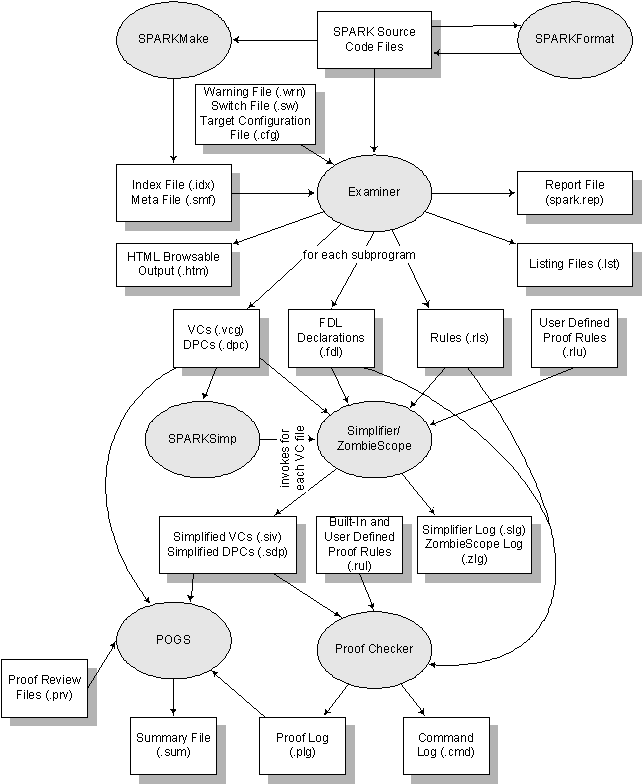
\includegraphics[height=7in]{figures/spark-tools.png}
    	\caption{Relationship of the Examiner and Proof Tools\protect\footnotemark.}
    \end{center}
\end{figure}
\footnotetext{http://docs.adacore.com/sparkdocs\-docs/Examiner\_UM.htm}



\section{SPARK Examiner}
\label{verification:examiner}

The main SPARK verification tool is Examiner. It supports several levels of analysis:
\begin{itemize}
	\item checking of SPARK language syntactic and static semantic rules
	\item data flow analysis
	\item data and information flow analysis
	\item formal program verification via generation of verification conditions
	\item proof of absence of run-time errors
	\item dead path analysis
\end{itemize}

There is also an option to make the Examiner perform syntax checks only. Using this option on a source file does not require access to any other units on which the file depends, so files can be syntax checked on an individual basis. This allows any syntax errors to be corrected before the file is included in a complex examination.  This option must only be used as a pre-processor: the absence of syntax errors does NOT indicate that the source text is a legal SPARK program. \cite{Examiner:Online} (THIS PART IS COPY AND PASTE FROM Examiner doc - is it ok?)

Put here some examples: method without contract, examine, add specification, pass Examiner.

During implementation, code was regularly checked using SPARK Examiner.

What is very important, Examiner can perform data and information analysis of Ravenscar programs in exactly the same manner as for sequential programs \cite{Ravenscar:Online}. Unfortunately it does not allow protected objects in proof annotations (pre- and post-conditions).

When some parts of the system are written in full Ada (with non-valid SPARK constructs), then Examiner returns error. Ada parts can be excluded from Examiner analysis using \lstinline{--# hide} annotation. The, only warning \lstinline{10 - The body of subprogram Main is hidden - hidden text is ignored by the Examiner.} is returned by Examiner.

Examiner use SPARK index file to locate files necessary for verification. \cite{Barnes:Book}

Examiner can be used with \lstinline{spark} command and appropriate flags described in Examiner Manual \cite{Examiner:Online}.

%http://docs.adacore.com/sparkdocs-docs/SPARK_GPS.htm
%[screenshot - take from 721 paper]
To use Examiner in GNAT Programming Studio:
\begin{itemize}
	\item Run SPARK Make (right click on project / SPARK / SPARK Make)
	\item Set SPARK index file (to spark.idx generated by SPARKMake) [add photo from 721 paper]
	\item (optionally) set configuration file (Standard.ads)
	\item Choose appropriate version of SPARK (95 or 2005)
	\item Choose mode: Sequential (for single tasking programs) or Ravenscar (for multitasking programs)
\end{itemize}

To generate verification conditions (VCs), the \lstinline{-vcg} switch has to be used. It can be set in GNAT Programming Studio (Project / Edit project properties / Switches / Examiner / Generate VCs).
In addition to verification conditions, Examiner can check dead path conjectures. It checks, whether all of the program is useful. To generate dead path conjectures, the \lstinline{-dpc} switch has to be used. It can be also set in GNAT Programming Studio (Project / Edit project properties / Switches / Examiner / Generate DPCs).


\subsection{Flow analysis}
\label{verification:examiner:flowanalysis}
%http://www.cs.swan.ac.uk/~csetzer/lectures/critsys/09/critsysfinal2.pdf
There are two types of flow analysis:
\begin{itemize}
	\item Data flow analysis:
	\begin{itemize}
		\item Checks input/output behavior of parameters and variables.
		\item Checks initialization of variables.
		\item Checks that changed and imported variables are used later (possibly as output variables).
	\end{itemize}
	\item Information flow analysis - verifies interdependencies between variables.
\end{itemize}

In data flow analysis, Examiner checks if input parameters are not modified, but used at least once (in at least one branch of program). In the same factor, output parameters cannot be read (before initialization) and has to be initialized (in all branches of program). Input/output parameters has to be both read and write (changed). In similar way, Examiner verify the global variables (specified in annotations). Functions can use only input parameters and can only read global variables. Therefore functions do not have side effects. 

Global variables defined in package body (thus private) has to be declared by \lstinline{--# own} annotation in package specification. If variable is also initialized, \lstinline{--# initializes} annotation has to be used. In Ada, to use package in another package, \lstinline{with} clause has to be used. In SPARK Ada, additionally \lstinline{--# inherits} annotation has to be specified.

In information flow analysis, dependencies between variables are analyzed. These dependencies are specified by \lstinline{--# derives} annotation.


\subsection{Verification conditions}
\label{verification:examiner:vc}

To generate verification conditions, two kinds of annotations are relevant for Examiner:
\begin{itemize}
	\item pre-conditions: \lstinline{--# pre}
	\item post-conditions: \lstinline{--# post}
\end{itemize}

Notion of pre- and post-conditions represents Hoare logic. More precisely, Hoare triple: 

\begin{equation} \label{eq:hoare_triple}
	\{P\} C \{Q\}
\end{equation}

P and Q are assertions. C is a command (action) performed between them. P is pre-condition and Q is post-condition.

Additionally, assertions (\lstinline{--# assert}) and checks (\lstinline{--# check}) can be specified in procedure body. Then additional verification conditions are generated.

Functions does not have side effects (as stated in \ref{verification:examiner:flowanalysis}), thus only pre-condition can be applied. However, there is annotation \lstinline{--# return}, which specify function return value.

Verification conditions are generated depended on number of paths in subprogram. Analysis are perform backwards, in other words: we start from post-conditions and consider what must holds before. Flow analysis is well described in chapter 11 of Barnes' book \cite{Barnes:Book}.



\section{SPARK Simplifier}
\label{verification:simplifier}

Simplifier can discharge (prove correctness) of verification conditions (VCs) generated by Examiner, but not proved by Examiner. \cite{Simplifier:Online} 



\section{ZombieScope}
\label{verification:zombiescope}

ZombieScope is a SPARK tool, that analyses SPARK code to find dead paths, i.e. paths through the code that can never be executed.


\section{Victor}
\label{verification:victor}

Victor is a tool to translate SPARK verification conditions (VCs), as generated by the Examiner, into SMT-LIB (file format used to communicate with SMT solvers). \cite{Victor:Online} SMT (Satisfiability Modulo Theories) solver is a tool...
experimental feature
Integrated with SPARKSimp (by -victor flag) and POGS.


\section{Proof Checker}
\label{verification:proofchecker}

% Barnes' book: 12.12
Only mention. It is hardcore.

\section{SPARKSimp Utility}
\label{verification:sparksimp}
SPARKSimp is a simple "make" style tool for the SPARK analysis tools. Currently, it supports the Simplifier, ZombieScope and ViCToR. It applies the Simplifier (and ViCToR, if requested, please see the Victor\_Wrapper user manual \cite{Victor:Online} for more information) to all .vcg files and ZombieScope to all .dpc files it finds in a directory tree. \cite{SPARKSimp:Online} 



\section{Proof Obligation Summarizer (POGS)}
\label{verification:pogs}

The Proof ObliGation Summarizer tool (POGS) reads and understands the structure of the verification condition files. It reports the status of proofs and dead path analyses in a human-readable form. \cite{POGS:Online}


\section{Example verification}
\label{verification:example}

An overview of verification contracts and annotations can be found in chapter 12 of Barnes' book \cite{Barnes:Book}.
On Odometer or RateController of PCA Pump?

\section{Verification of PCA Pump}
\label{verification:pcapump}

Examine(F8) -> Simplifier --> POGS.

4 warnings:
Warning 402 - Default assertion planted to cut loop.

solution:
\lstinline{--# assert I > 1 -> TheStoredData(I-1) = TheStoredData(I);}
\lstinline{--# assert I > 1 -> Result >= TheStoredData(I-1);}
\lstinline{--# assert true; // add BLESS assertions? then resolve warning 402?}
\lstinline{--# assert true; // add BLESS assertions? then resolve warning 402?}


Verification of main.adb

\begin{lstlisting}
main.adb:4:10: Warning 391 - If the identifier Text_IO represents a package which contains a task or an interrupt handler then the partition-level analysis performed by the Examiner will be incomplete.  Such packages must be inherited as well as withed.
main.adb:6:10: Warning 391 - If the identifier Float_Text_IO represents a package which contains a task or an interrupt handler then the partition-level analysis performed by the Examiner will be incomplete.  Such packages must be inherited as well as withed.
main.adb:102:5: Warning  10 - The body of subprogram Main is hidden - hidden text is ignored by the Examiner.
main.adb:14:49: Flow Error 602 - The undefined initial value of Pca_Pump.Operate may be used in the derivation of Pca_Pump.State.
main.adb:14:49: Flow Error 602 - The undefined initial value of Pca_Pump.Fluid_Pulses may be used in the derivation of Pca_Pump.State.
main.adb:14:49: Flow Error 602 - The undefined initial value of Pca_Pump.Prescription may be used in the derivation of Pca_Pump.State.
main.adb:14:49: Flow Error 602 - The undefined initial value of Pca_Pump.Clinician_Bolus_Paused may be used in the derivation of Pca_Pump.State.
main.adb:14:49: Flow Error 602 - The undefined initial value of Pca_Pump.Clinician_Bolus_Duration may be used in the derivation of Pca_Pump.State.
main.adb:14:49: Flow Error  37 - The updating of variable Pca_Pump.Operate by a task or interrupt handler has been omitted from the partition annotation.
main.adb:14:49: Flow Error  37 - The updating of variable Pca_Pump.Fluid_Pulses by a task or interrupt handler has been omitted from the partition annotation.
main.adb:14:49: Flow Error  37 - The updating of variable Pca_Pump.Clinician_Bolus_Paused by a task or interrupt handler has been omitted from the partition annotation.
main.adb:14:49: Flow Error  36 - The referencing of variable Pca_Pump.Operate by a task or interrupt handler has been omitted from the partition annotation.
main.adb:14:49: Flow Error  36 - The referencing of variable Pca_Pump.Fluid_Pulses by a task or interrupt handler has been omitted from the partition annotation.
main.adb:14:49: Flow Error  36 - The referencing of variable Pca_Pump.Prescription by a task or interrupt handler has been omitted from the partition annotation.
main.adb:14:49: Flow Error  36 - The referencing of variable Pca_Pump.Clinician_Bolus_Paused by a task or interrupt handler has been omitted from the partition annotation.
main.adb:14:49: Flow Error  36 - The referencing of variable Pca_Pump.Clinician_Bolus_Duration by a task or interrupt handler has been omitted from the partition annotation.
/Volumes/External/VMS/shared/aadl-medical/pca-pump-beagleboard/pca_ravenscar/main.adb:1:1: Warning - VC generation requested but no bodies presented. No VCs generated.
\end{lstlisting}





\section{AUnit tests}
\label{verification:aunit}
- test incrementing array
- test moving array (Pulse does not change dosed amount)
- test prescription setters and getters
- test state machine
	* change to bolus mode
	* change to KVO rate
	* etc.



\section{gnatPROVE?}
\label{verification:gnatprove}

There is a new tool set "gnatPROVE" for SPARK 2014. It was not used because PCA Pump was developed in SPARK 2005.
I CAN TRANSLATE SOME SINGLE FUNCTIONS AND USE GNAT PROVE TO VERIFY?
